\chapter{Implementation}
\label{chap:Implementation}

In this chapter we will expand on the process of implementing our proof of concept.
Before we can discuss the actual work of implementing the architecture we need to define the developing environment.
This will include an introduction of the software libraries Tinzenite will base some of its functionality on.

\section{Tools and Environment}
\label{sec:Tools and Environment}

In this section we will discuss the tools we used to build the software proof of concept.
This includes libraries we utilized and the software used to write the programs.

\subsection{Golang}
\label{sub:Golang}

As previously stated the proof of concept implementation will be developed using the programming language Golang.
We will make full use of a range of features which we will briefly highlight in the following.

A Golang program will compile into a single native executable file, with statically linked dependencies.
Cross compilation is available to all major operating systems and processor architectures.
Unlike for example Java Golang does not depend on a virtual machine to run resulting in performance that is near to natively compiled C code.
Furthermore Golang is not an object oriented language and based more on C than any other language.
Golang is statically typed and garbage collected.
This gives us type safety and removes the need to manage the memory ourselves.
For a developer coming from Java a large standard library helps to ease the transition: Golang offers such a standard library.
We found writing Golang code to be less verbose than Java code for the same task while not being any harder to comprehend.

Golang handles errors and exceptions differently in comparison to Java.
While in Java error handling is done explicitly via exceptions, Golang uses simple return values to signal errors.
This poses less of a problem than it may initially seem to as Golang functions can return multiple values.
Furthermore Golang exposes and allows working with object pointers.
Concurrency is also directly built into the language via so called \textit{"go routines"} and channels.
Unlike Java which builds objects with class inheritance, Golang uses composition and interfaces to build objects.
Building on this Golang does not even require the declaration of which interfaces an object implements -- having the method of an interface means that that object implements the interface.

Golang also lacks a few features, notably generics and function overloading.
We found these to be relatively easy to work around, although the lack of generics leads to an increase in redundant boilerplate code in some instances.
A possibly higher hurdle is the lack of fine granular permissions: unlike Java Golang knows only private and public variables and functions, indicated by their names beginning with a lowercase or respectively uppercase letter.

As to the development environment surrounding Golang only a few specifics should be noted.
A very nice feature is that packaging is directly built on top of version control systems.
This means for example that \textit{"\href{https://github.com/xamino/tox-dynboot}{github.com/xamino/tox-dynboot}"} is both the package path and the URL where the package can be retrieved from.
Within the code the package would be referenced by the name, commonly the last part of the package path.
Golang also requires all code to be formatted according to its specifications which results in improved readability across different packages.
A variety of tools are directly built into the development suite, including a tool to fetch packages from their path and a tool for vetting and formatting Golang code.

\subsection{JSON}
\label{sub:JSON}

\begin{listing}[H]
    \begin{lstlisting}[language=golang,firstnumber=0]
type Message struct {
    Address string
    Subject string `json:"omitempty"`
    Content string `json:"Message"`
    read    bool
}
    \end{lstlisting}
    \begin{lstlisting}[language=json,firstnumber=0]
{
    "Address":"192.168.178.100",
    "Message":"Log in successful!"
}
    \end{lstlisting}
\caption[Golang JSON Example]{
    An example Golang struct with tags and its corresponding JSON representation.
    Note that \textit{"Subject"} is missing from the JSON due to the \textit{"omitempty"} tag and \textit{"read"} due to it being private.
    Also note that \textit{"Content"} has been renamed to \textit{"Message"}.
}
\label{golang:json_example}
\end{listing}

Since the underlying Tox channel is built for text based messaging we propose to implement all peer to peer communication as a human readable messaging format.
We will therefore utilize Javascript object notation, short JSON, as a machine readable message format while retaining easy readability for developers.
As an added bonus Golang has support for converting objects by default thanks to the standard libraries.
The generation of JSON can be fine tuned by utilizing in-language tagging.
Listing~\ref{golang:json_example} shows a very simple example.

\subsection{Tox Binding}
\label{sub:Tox Binding}

As stated in various instances before we will be building all peer to peer communication on the Tox core library~\cite{web:site:github:toxcore}.
Since the library is implemented with the C programming language we require a Golang wrapper for it.
Instead of implementing one ourselves which would have cost us a large amount of development time we chose to use an existing one.
With some research we chose the wrapper written and provided by codedust via Github~\cite{web:site:github:gotox}.

At the start of the Tinzenite implementation this wrapper still lacked one significant feature that Tinzenite required, namely the capability of sending and receiving files.
However a feature request~\cite{web:site:github:file_issue} was submitted and promptly implemented by the maintainer.
The maintainer was also forthcoming in helping us solve bugs and problems with our usage of the wrapper for which we are grateful.

\subsection{Hadoop Client Binding}
\label{sub:Hadoop Client Binding}

For the encrypted peer we required an implementation for a client for the Hadoop distributed file system.
We chose the implementation by the Github user colinmarc.
Notably we used the branch that adds write support~\cite{web:site:github:hdfs}.
This library is not a wrapper but an implementation of a HDFS client written in Golang.

\subsection{Environment}
\label{sub:Environment}

Tinzenite was implemented on the Arch Linux distribution Antergos~\cite{web:site:antergos}, specifically the amd64 flavor.
The Golang environment was set up using the corresponding Arch package~\cite{web:site:arch_go}.
We used the Golang tools provided by the package to compile our work.
The code itself was written using the Atom text editor~\cite{web:site:atom} with a variety of extensions, most notably the support extensions for Golang.
Git~\cite{web:site:git} was used for the version control system, with a hosted repository on Github here~\cite{web:site:github:tinzenite}.

\section{Software Structure}
\label{sec:Software Structure}

Tinzenite was developed not as a single package but as a package collection where each package covers some part of the complete scope.
In this section we will discuss the general layout of the packages and how they depend on one another.
Figure~\ref{fig:implementation_structure} shows an informal diagram of the structure.
All packages have their own repository on Github~\cite{web:site:github:tinzenite}.
\newpage

\begin{figure}[htp]
\centering
    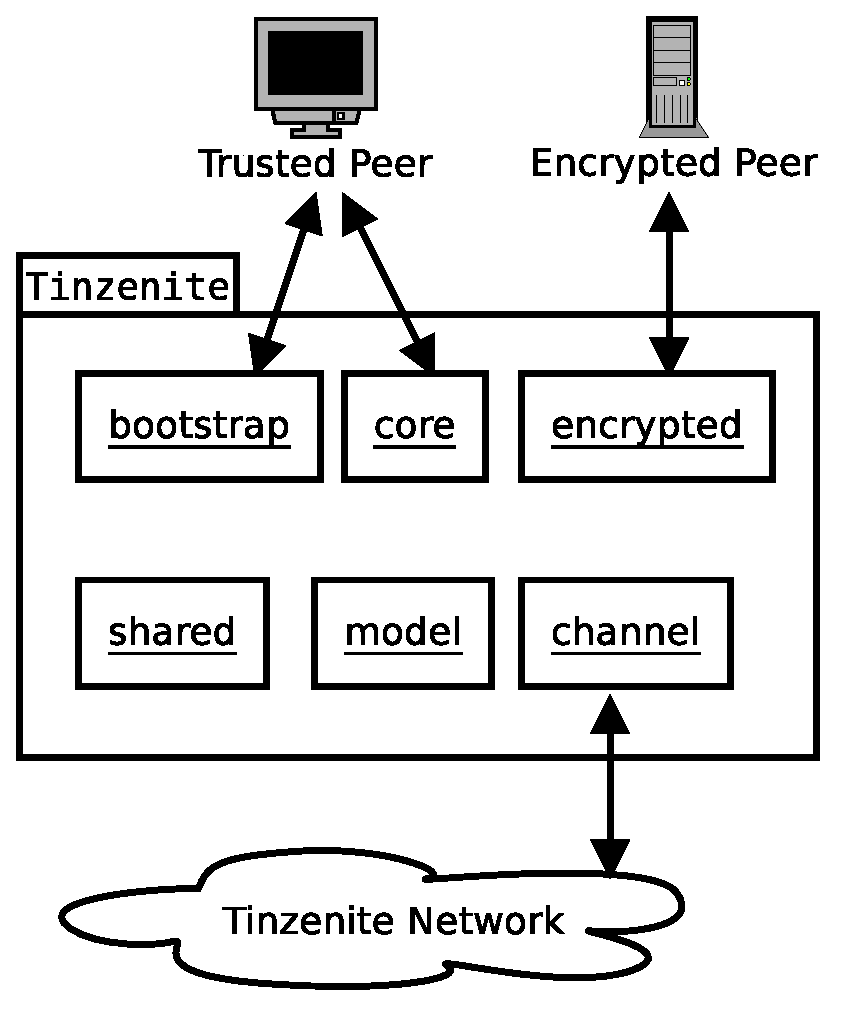
\includegraphics[width=5cm]{diagram/topo_implementation}
\caption[Tinzenite Structure]{This diagram shows an informal representation of the package structure of our implementation.}
\label{fig:implementation_structure}
\end{figure}

\begin{description}[leftmargin=6em,style=nextline,noitemsep,nolistsep]
    \item[bootstrap]
        Contains the library for bootstrapping both encrypted and trusted peers to an existing Tinzenite network.
    \item[channel]
        Building on the Tox wrapper implements an abstract object for all Tox related communication code.
    \item[core]
        Implements the functionality for a trusted peer.
    \item[encrypted]
        Implements the functionality for an encrypted peer.
    \item[model]
        Contains the directory tracking code which manages a Tinzenite directory.
    \item[server]
        Built on the \emph{encrypted} package implements an example server program for an encrypted peer.
    \item[shared]
        Contains various shared objects used by multiple packages.
    \item[tin]
        Built on the \emph{core} package implements an example user program for a trusted peer.
\end{description}

We began the implementation with the \emph{model} and the \emph{channel} packages, then built the \emph{core} package on top of these.
At one point we began writing shared code into the \emph{shared} package for reuse.
The \emph{tin} package was added early on for testing and debugging purposes and grew alongside the trusted peer development.
Once the basic functions worked we implemented the \emph{bootstrap} package.
Then we built the \emph{encrypted} and \emph{server} packages to implement the encrypted peer.
Finally we adapted the \emph{bootstrap} package for both peer types.

\section{Highlights}
\label{sec:Highlights}

The following section will serve to discuss highlights of the implementation.
We will also expand on some aspects of the implemented functionality where we believe an expanded discussion is stimulating.

\subsection{Model}
\label{sub:Model}

The \emph{model} package contains the model object used by the trusted peer to manage a tracked directory.
Instances of the model can be created either by loading it from a JSON store or creating a new one.
The model itself does not actively update itself if the underlying directory changes: instead an update must be triggered by the utilizing code.
This allows the model to avoid having to employ file watchers.
It thus falls to the utilizing code to call the update method in regular intervals to ensure that the model remains up to date.

The initial version of the model object only used file hashes to check for modifications, according to the Tinzenite specifications.
For large files or a large amount of files this proved to be a very slow operation.
Thus we also store the modification time as written to the file system upon creation and modification of a file to the model.
This attribute is private to the model.
As long as the modification time has not changed we do not need to recalculate the hash as nothing has changed since the last check.
Thus the model is only required to recalculate the hash when the file actually has been modified.
This greatly speeds up the update detection phase.

Apart from reacting to direct directory changes the model object also allows remote updates to be applied.
Before a remote update can be applied a number of parameters must be checked -- therefore the model object offers a \texttt{CheckMessage} method that returns whether the update must be truly applied.
The update may be ignored for example if it has already been applied, or when it concerns an already completed removal as stated in section~\ref{subs:Remove}.
Any call to \texttt{ApplyUpdateMessage} should be preceded by applying this message check.
Note that we have moved most of the removal logic code to its own code file for easier comprehension.

Any application of an update may trigger a merge conflict.
This is signaled by the model via an error.
It is up to the caller to then handle the merge in a valid fashion, likely calling the model to apply resulting updates to the directory.
Tinzenite handles merge conflicts as part of the \emph{core} package.

\subsubsection{Ignoring Objects}
\label{subs:Ignoring Objects}

The \emph{model} package also implements the matcher object.
This object checks each directory for a \textit{".tinignore"} file and if it exists applies it to any model work on the directory.
The file containing these rules can be synchronized just as any other file at any level within a directory.
Any new objects detected by Tinzenite that are listed in this file will not be created within the model, effectively keeping it out of the Tinzenite network.
Since it may well happen that a \textit{".tinignore"} is created at a later point and thus introduces an uncertainty in handling the files to be ignored we propose a simple solution: the file is only ever applied for object creations.
Once a file has been created within the model it will be modified and deleted as any other file within the system, independent of whether it was or is to be ignored.

\begin{listing}[htp]
    \begin{lstlisting}[language=golang,firstnumber=0]
# DO NOT MODIFY!
/local
/temp
/receiving
/sending
    \end{lstlisting}
\caption[Meta Ignore File]{The \textit{".tinignore"} file contents for the \textit{".tinzenite"} directory. Note that it allows comments. In this example only directories are excluded. Files can be excluded too: lines starting without the slash are considered file ignore rules.}
\label{tinignore:meta}
\end{listing}

The \textit{".tinignore"} file is used in the \textit{".tinzenite"} directory to control which parts are synchronized and which not, as mentioned in section~\ref{sec:Meta Data}.
Listing~\ref{tinignore:meta} shows the contents of this \textit{".tinignore"} file.
Note that ignoring objects is supported within the complete Tinzenite directory: users that are so inclined can add such files themselves to control what objects Tinzenite synchronizes.
We added support for comments to improve readability for users.
The current implementation does not offer support for regular expressions or more advanced matching grammars, although these features should be comparatively simple to add.

\subsection{Channel}
\label{sub:Channel}

The \emph{channel} package wraps the Tox wrapper into the channel object via which all communication is sent.
The channel object makes use of callbacks to allow callers to react to incoming messages, file transfers, and other events.

Since the underlying Tox instance must be called in regular intervals, the channel object implements a background go routine that keeps Tox ticking.
To avoid locking up the Tox instance on callbacks, each callback is called asynchronously.
If a callback can result in a direct response that must be passed to the Tox instance, another method is available.

Tox requires bootstrapping to known nodes to connect to the Tox network.
This bootstrapping is different from the bootstrapping of peers we will discuss later.
The channel object makes sure that the Tox instance is bootstrapped to the Tox network if it is not connected as long as the channel is kept running.
We dynamically retrieve a list of available Tox nodes using a specially written package~\cite{web:site:github:tox-dynboot}.
This list is used to try to connect a given channel to the Tox network.

Unlike both the Tox instance and the Golang wrapper for it, the channel object wraps the file transmission nicely.
If a file transfer request is received it asks the utilizing code via a callback whether to accept the transfer or not.
If accepted it will again notify when the file has been successfully received or the transfer failed.
Tox itself handles file transfers in data blocks.
For our purposes the abstraction of this process greatly simplifies quite a lot of code that builds on file transfers.

The channel object furthermore offers a wide range of helpful methods that are not directly available from a Tox instance.
This includes handling all addresses as hexadecimal encoded strings versus byte arrays and a number of status functions.

\subsection{Tin Program}
\label{sub:Tin Program}

The \emph{tin} package is an example implementation of a trusted peer built on the \emph{core} package.
While a true client built on a stable Tinzenite version should interface with the user via a graphical user interface, we forewent this because of the increased development time.
Thus the Tin program is a simple command line interface based program.

It offers a range of flags to make a Tinzenite directory easier to manage.
Each instance of Tin should run for a single trusted Tinzenite peer.
Additionally the program can also be used to create new peers and bootstrap them to the Tinzenite network.
In the case of bootstrapping an encrypted peer the program will exit on successful completion.
For trusted peers the program will immediately continue by running the directory.
If a trusted peer receives a bootstrapping request it asks the user to validate the given peer address and requested trust level.

The program also automatically updates the local directory, requests remote updates, and synchronizes with available encrypted peers at certain intervals.
This serves to prove that Tinzenite can run completely without user input.
In fact apart from setting up a peer the synchronization runs fully without user input, even if merge conflicts arise.
Care was taken to ensure that the entire program could run using as little resources as possible.
Currently the program runs with negligible CPU and RAM usage even though synchronizing regularly.
The only truly expensive operation where the program requires more performance is for hash generation and encryption when handling files.
On an Intel Core i5-4440 with 4 physical cores at 3.1 GHz, each instance of Tin remains under 1\% CPU and around 9 MB of RAM usage over a prolonged period of time when no update operations beyond model synchronization are executed.

The \emph{core} package itself wraps the complete trusted peer code.
Basically it uses the model object and the channel object to offer all trusted peer functionality.
Notably it also implements how Tinzenite handles merge conflicts.
For software written against it the core package exposes a Tinzenite object with which the trusted peer can be controlled.

\subsection{Bootstrap}
\label{sub:Bootstrap}

Initially we planned to include the bootstrapping code directly within the tin and core packages.
However the differences in how a peer must react to incoming messages and transfers would have greatly increased the already substantial code complexity of these packages.
Therefore we moved all bootstrapping related code into its own package.
This has the large advantage that programs can easily implement just bootstrapping if required to without needing any further package imports.

The basic function of bootstrapping is relatively simple.
It requires the address of the trusted peer to connect to and sends a Tox friend request to it to initiate the connection.
Once the friend request has been accepted and the trusted peer has been connected the actual bootstrapping takes place.
For a new trusted peer that includes fetching the complete current state of the directory.
Once the transfers are complete the bootstrapping code finishes and the directory can now be started as a normal trusted peer.

The bootstrap package was mainly implemented in one sitting and serves as a proof of concept that the previously implemented code for the trusted peer program could be reused easily.
Apart from bug fixes we only had to update it once we implemented the encrypted peer functionality.

\subsection{Server Program}
\label{sub:Server Program}

Much like the Tin software the \emph{server} package provides an implementation for the \emph{encrypted} package.
It offers a command line interface program for creating and running an encrypted peer.

\begin{listing}[htp]
    \begin{lstlisting}[language=golang,firstnumber=0]
package encrypted

type Storage interface {
	Store(key string, data []byte) error
	Retrieve(key string) ([]byte, error)
	Remove(key string) error
}
    \end{lstlisting}
\caption[Encrypted Storage Interface]{The storage interface that the encrypted peer must implement to use the \emph{encrypted} package. Comments have been removed.}
\label{golang:storage_interface}
\end{listing}

Adding encrypted peers to Tinzenite required two tasks to be successful: the implementation of the encrypted peer and the extension of the trusted peer to be capable of utilizing it.
The first task of implementing the encrypted peer proved to be comparatively simple.
Basically all it has to do is offer a lock to any single trusted peer and the, when locked, allow the fetching and retrieval of files.
Most files the encrypted peer handles are user data files.
One of the goals for this thesis was to support writing these files to the Hadoop distributed file system.
Therefore we implemented the encrypted peer so that all user files are written with a specified storage interface as seen in listing~\ref{golang:storage_interface}.
However this storage interface is not used for all files.
The authentication file and the peer files are required to exist unencrypted and are required for the encrypted peer to run correctly.
Therefore these files are written to disk within the \textit{"org"} directory\footnote{The encrypted peer does not share the directory structure of a trusted peer. The reason for this is that an encrypted peer lacks many of the features that went into the design of the \textit{".tinzenite"} directory. Thus a simpler, flatter structure was chosen.}.

The storage interface allows encrypted clients, such as the \emph{server} package provides an example of, to interface with any storage interface a developer requires it to.
For this thesis we implemented two versions of the interface for the server program.
First for debugging and personal use we implemented a version of the interface that simply writes all data to disk, named as the key of the data.
Retrieval looks up the file by checking for the existence of a file named as the given key and returns the associated data.
Then we implemented the actual Hadoop capable version of the interface.
Our version of the interface creates a connection to a Hadoop distributed file system when initiating.
All further file accesses will then be handled as operations on the Hadoop cluster.

Once the encrypted peer was implemented we turned to the more complex task of integrating encrypted peers into the capabilities of the trusted peer.
This meant modifying the core package so that trusted peers could differentiate between trusted and encrypted peers and communicate with each accordingly.
Upon receiving a message the trusted peer always first checks whether the message came from an encrypted peer or a trusted peer on a case by case basis.
We do this by checking the address of the sender against the known peer list and ensuring that trusted peers have been authenticated.
The message is then passed on to the specific logic for the type of peer.

The logic for handling an encrypted peer comes down to a relatively simple process.
Upon successful locking an encrypted peer to itself, the trusted peer requests the encrypted model.
If the encrypted peer responds with a notification that the file doesn't exist the encrypted peer is considered empty and the logic skips to uploading the current state of the trusted peer.

If a model is received the trusted peer must first compare the remote model against its own model to check for changes.
Unknown updates of the encrypted peer are applied to the trusted peer by fetching the necessary files.
Once this is complete the next step is to update the encrypted peer to the state of the trusted peer.
Updates that the trusted peer has but the encrypted peer lacks are uploaded and finally the current model is encrypted and also uploaded.
Then the encrypted peer is unlocked so that other trusted peers can access it too.

\subsection{Golang Issues}
\label{sub:Golang Issues}

We encountered a small amount of gotchas due to our unfamiliarity with the Golang language.
In the interest of full disclosure we will use this section to briefly touch on these matters.

Tinzenite builds heavily on the standard libraries included with the language.
Since Golang is still a relatively new language we expected to encounter bugs and issues as we implemented Tinzenite.
However we only encountered a single bug.
It effected the generation of a random integer for issuing a challenge.
After creating a valid random \texttt{int64} value for the challenge we required a byte slice representation of the variable to encrypt it.
We had to determine the size of the byte slice so that the variable could be stored in it.
Research lead us to believe that utilizing the \texttt{byte.Size} method would allow us to make the byte slice just large enough to contain the random number.
But the method always returned incorrect values.
Our workaround is to simply create the slice large enough for all possible values at a small memory cost.

The good performance of Tinzenite was initially not the case.
First versions of the trusted peer had a slow memory and processing leak resulting in steadily rising CPU and RAM usage until the host computer killed the process after a few minutes.
We tracked this down to our usage of an endlessly running go routine utilizing \texttt{time.Tick} to run in intervals.
As stated in the method documentation the underlying \texttt{Ticker} can not be closed, thus resulting in a leak~\cite{web:site:golang:time:tick}.
We worked around this issue by simply reusing the timing objects instead of recreating new ones within every interval.

Another problem was that we had no way to determine the type of \texttt{struct} we required to parse incoming JSON messages.
Thus we implemented a \textit{"Type"} attribute for all messages which we use to determine the correct type of the message.
Golang's composition was not a viable way of solving this to our satisfaction since all message objects did not have any differing methods.
The correct way to do this is to parse the incoming messages to an empty interface which is valid for all types.
The type can then be checked and the message can then be casted.

\begin{listing}[htp]
    \begin{lstlisting}[language=golang,firstnumber=0]
type MsgType int

const (
	MsgNone MsgType = iota
	MsgUpdate
	MsgRequest
	MsgNotify
	MsgLock
	MsgPush
	MsgChallenge
)
    \end{lstlisting}
\caption[Golang Enum Example]{One of the enumerations we defined for Tinzenite. Note that for brevity we removed the comments.}
\label{golang:enum_example}
\end{listing}

For the defined messages that Tinzenite uses we heavily relied on enumerations for setting values.
Coming from Java we expected to find similar \texttt{enum} functionality in Golang.
This did not prove to be the case.
Golang lacks a specific implementation of enumerations but does allow for something similar using the \texttt{const} and \texttt{iota} keywords for specified variable types.
An example can be seen in listing~\ref{golang:enum_example}.
Our largest issue with this was that when converting these enumeration similes to JSON instead of the name of the enumeration the number value was output due to Golang seeing them as number value variables.
Thus instead of having JSON where each enumeration was easily interpretable we had values such as \texttt{"MsgType":1} where what we wanted was \texttt{"MsgType":"update"}.
The solution to this requires a lot of boilerplate code since Golang does not support generics at this point in time.
For each defined enumeration type we had to write custom \texttt{MarshalJSON} and \texttt{UnmarshalJSON} methods, which we did where applicable.

\section{Security}
\label{sec:Security}

This section will discuss the scheme used to encrypt and decrypt files within Tinzenite and how the keys are stored and shared.
Generally speaking Tinzenite uses two encryption layers to ensure file security.
We will also briefly discuss the exact method we utilize for the challenge response algorithm.

The encryption scheme we used in Tinzenite is the NaCl library~\cite{bernstein2012security} through its interoperable Golang package~\cite{web:site:golang:box}.% interoperable is spelled correctly
From this package we utilize just three methods: \texttt{GenerateKey}, \texttt{Open}, and \texttt{Seal}.
They are used to generate encryption keys, decrypt data, and encrypt data.

\subsection{File Encryption}
\label{sub:File Encryption}

Every Tinzenite network generates a single permanent key pair which is used to encrypt and decrypt data.
Each peer upon creation generates these keys but will overwrite them with the network's keys if connected to an existing network during bootstrapping to ensure that each Tinzenite peer uses the same keys.
Otherwise peers could not share encrypted peers between themselves as each would use a different set of encryption keys.
The keys themselves are generated using the cryptographically secure random number generation provided by the host operating system to ensure that they are truly random.

File data is encrypted before sending it and decrypted after receiving it when exchanging data with encrypted peers.
To encrypt and decrypt data via NaCl we require an associated nonce which must be atomic but unique to every encryption decryption cycle.
We require a way to store and retrieve the nonce for each encrypted data blob.
Instead of writing the nonce somewhere else we opted to prepend the nonce to the encrypted data. % prepend is spelled correctly
Thus the first 24 bytes of every encrypted file contain the nonce required to decrypt it again.
Figure~\ref{fig:enc_algo} shows an example of how this works.

\begin{figure}[htp]
\centering
    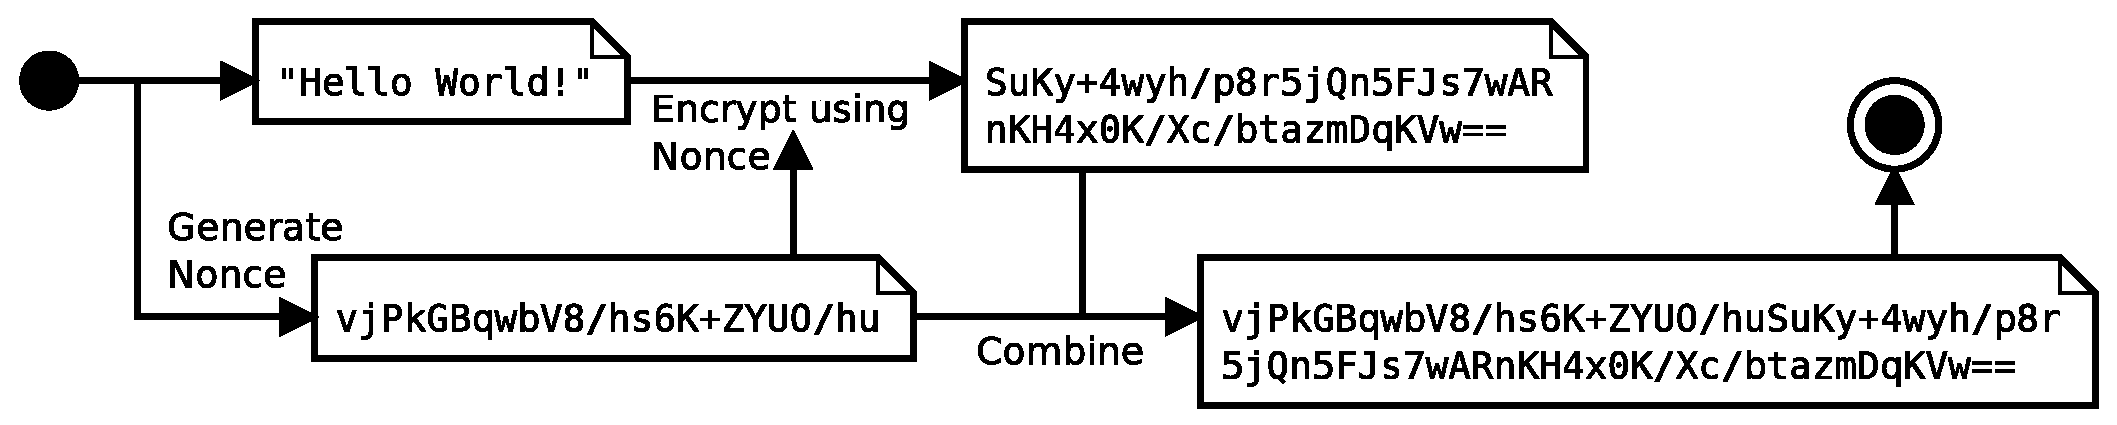
\includegraphics[width=14cm]{diagram/enc_algo}
\caption[Encryption Example]{This diagram shows an example of how the nonce is integrated into the data for an encrypted message.}
\label{fig:enc_algo}
\end{figure}

When decrypting data we must thus remove the nonce from the data before decrypting it.
Since the decryption requires the nonce we can simply use it directly.
The nonce is then discarded and the decrypted data is ready to use.

\subsection{Key Encryption}
\label{sub:Key Encryption}

Now that all data can be encrypted and decrypted correctly the question turns to how to store the corresponding keys safely.
At first glance a simple solution would be to synchronize the keys only between trusted peers.
However this would not allow an implementation for a web peer as described in section~\ref{sub:Web Interface Peer}.
A temporary peer could not request the keys because it could not authenticate itself.
Thus the keys must be stored alongside the encrypted data.

It is immediately obvious that simply storing the keys in plain text next to the encrypted data offers no security.
So the keys must be encrypted too but with another set of keys.
The question then is where to store these keys for encrypting the encryption keys.
Since Tinzenite should be user friendly and secure we opted for an interesting algorithm for generating the keys that unlock the actual encryption keys.
To differentiate the two different sets of keys we will reference the encryption keys which are used to encrypt and decrypt the other keys as the box keys.

On creating a Tinzenite network the user is asked for a password or better yet a passphrase~\cite{web:site:xkcd:pwd_strength}.
We then use this passphrase to generate the box keys used to encrypt the encryption keys.
Now the encryption keys can be encrypted with the box keys and safely transmitted to both trusted and encrypted peers.
The question now arises how other trusted peers can retrieve the box keys.

The answer lies in the user given passphrase and the way the box keys are generated.
Every trusted peer must be unlocked by the user with the passphrase\footnote{Note that the trusted peer should store the passphrase once the user has entered it to avoid needless repetition and to increase the ease of use for future accesses.} to decrypt the encrypted peers.
This passphrase is not stored somewhere in the Tinzenite network for a directory, meaning an attacker has to guess it.

\begin{listing}[htp]
    \begin{lstlisting}[language=golang,firstnumber=0]
func (a *Authentication) convertPassword(password string) (public *[32]byte, private *[32]byte, err error) {
	hasher := fnv.New64a()
	hasher.Write([]byte(password))
	seed := int64(hasher.Sum64())
	seededRandom := unsecure.New(unsecure.NewSource(seed))
	wrapper := staticRandom{random: seededRandom}
	public, private, err = box.GenerateKey(wrapper)
	if err != nil {
		return nil, nil, err
	}
	return public, private, nil
}
    \end{lstlisting}
\caption[Golang Box Key Generation]{The method for generating the box keys from a given passphrase. The \texttt{staticRandom} object is a wrapper for the random source so that it can be passed to the \texttt{box.GenerateKey} as the correct type. It is defined elsewhere.}
\label{golang:boxkey_gen}
\end{listing}

The box keys are then generated from the passphrase.
First we hash the passphrase to a number hash value.
This number hash is then used to seed a pseudo random number generator.
We then utilize this deterministic random number generator to create the box encryption keys.
Listing~\ref{golang:boxkey_gen} shows the entire code required to generate the box keys from a given passphrase.

This method of storing the encryption keys has a few advantages over other approaches.
An important advantage of decoupling the passphrase from the encryption keys via the box keys is that this allows the user to change his passphrase if desired.
Tinzenite must then only decrypt the encryption keys with the old passphrase and encrypt them with the new one.
The update will then propagate through the network\footnote{Note that we make no provisions for invalidating old passphrases since this would require substantially more encryption work and would most likely not be enforceable.}.
Encrypted peers do not need to be encrypted anew since the actual encryption keys remain the same.
Another advantage is that the entire encryption process is tied to a passphrase that is simple to remember and the user can freely assign and modify.
Apart from said passphrase the user must do nothing to ensure full encryption security for the Tinzenite network.

\subsection{Challenge Response}
\label{sub:Challenge Response}

The challenge response we use in Tinzenite is built on a very simple challenge.
For each challenge we generate a random number and locally store it, then encrypt it with the data encryption keys and send it to the other peer.
This responding peer decrypts the message and retrieves the number.
It then increments it by one, encrypts its answer, and sends it back\footnote{What we actually do with the number is irrelevant as long as both sides of the challenge response algorithm use the same operation. The only property the operation must have is that it is sufficient to prove that both sides could read the unencrypted number and work on it.}.
If the received number is one value higher than the stored number, the challenge response is valid.

The challenging peer can thus be satisfied that the other peer is valid because it proved that it could validly decrypt and encrypt the correct values.
The responding peer knows the challenging peer is authenticated because it could issue a valid challenge for the network data encryption keys.
In all the challenge response mechanism for Tinzenite requires only two messages and a single random number to validate both sides of the exchange.
